\chapter{Task planner}
\label{ch:task_planner}
In this chapter the general framework adopted is discussed, proposing a suitable task planner. After the  review of the current state of the art of task planners, a proper planner is chosen and then a suitable description to the table clearing problem is discussed.
\section{Task Planners Review}
As already seen in chapter \ref{ch:state_of_the_art} there exist different kind of planners and they can be grouped in three main categories:
\begin{enumerate}
\item classical planners
\item hierarchical planners
\item probabilistic planners
\end{enumerate}
\textbf{Classical planners}, as suggested by the name, are the more classical and easy to use. They are characterized by environments which are fully observable, deterministic, finite and static (changes happen only when the agent acts) and discrete (in time, actions, objects...) \citep{artificialIntelligence}.
A deterministic problem is generally formulated as a $6$-tuple $\Pi=\langle S^d, s_o^d, G^d, A^d, T^d, c^d \rangle$ \cite{little2007probabilistic}, where:
\begin{itemize}
\item $S^d$ is a finite set of states;
\item $s_o^d \in S^d$ is an initial state;
\item $G^d \in S^d$ is a goal state;
\item $A^d(s)$ is a set of applicable actions for each $s \in S^d$;
\item $T^d(a,s) \in S^d$ is a deterministic transition function for all actions $a \in A^d(s)$ and states $ s \in S^d$;
\item $c^d(a)$ is the cost to apply action $a$. 
\end{itemize}
The solutions, or trajectories, $\tau_i$ are sequences of actions applicable from the initial state until the goal state. The cost of a trajectory $C(\tau_i)$ is the sum of the cost of the actions of the trajectory $\sum_{a \in \tau} c^d(a)$. The optimal solution is the solution with less cost: $\tau^* = \min_{\tau_i} c(\tau_i)$. A very well known classic planner is the Fast Downward planner \cite{helmert2006fast}.

\textbf{Hierarchical planning}, also called \textit{Hierarchical Task Network}(HTN), works in a similar way to how it is believed that human planning 
works \citep{marthi2007angelic}. It is based on a reduction of the problem. The planner recursively decomposes tasks into subtasks, stopping when it reaches primitive tasks that can be performed directly by planning operators. This kind of planner needs to have a set of methods, where each method is a schema for decomposing a particular kind of task into a set of subtasks \citep{shopDescription}. For this kind of planning technique a well known planner is JSHOP2 \cite{JSHOP2}.

\textbf{Probabilistic planning} is a planning technique which consider that the environment is not deterministic but probabilistic. So the actions have a certain probability to obtain a certain state, and given an initial and final state the planner  finds the solution path with the highest probability. A well known example on which this kind of planners are build on is the Markov Decision Process. A probabilistic problem is generally formulated as a $6$-tuple $\Pi=\langle S, s_o, G, O, T, A \rangle$ \cite{little2007probabilistic}, where:
\begin{itemize}
\item $S$ is a finite set of states;
\item $s_o \in S$ is the initial state;
\item $G \in S$ is a goal state;
\item $O$ is the set of outcomes, the probability of $o \in O$ is $Pr(o)$;
\item $T(o,s) \in S$ is a (total) deterministic transition function for all outcomes $o \in O$ and states $s\in S$;
\item $A(s)$ is a set of applicable actions for each $s \in S$, coupled to a function $out(a) \subseteq O$ mapping each action to a set of outcomes in such a way that 
\begin{itemize}
\item each outcome $o \in O$ belongs exactly to one action $act(o)$;
\item $\sum_{o \in out(a)} Pr(o) = 1$ for all $a$.
\end{itemize}
\end{itemize}
In this case the optimal solution is the one with the highest probability. In this category two famous probabilistic planners are Gourmand \cite{Gourmand} and PROST \cite{PROST}.

\section{Planner}
The problem this thesis is facing could be resolved by several approaches by using planners from all the categories. We have already seen that such a problem involves geometric constraints and those cannot be considered directly by the planner using a ready to use state of the art planner, that would imply a designing of a new planner. Moreover using a hybrid planner is also time consuming, so we decided to focuse on a strategy that would let us to use already existing planners. This way involves working with symbolic predicates. Symbolic predicates are predicates which can be true or false, and they will be introduced more in detail in the next sections. 

The problem moreover involves a big amount of uncertainty due to the interaction of the robot with the environment. When the robot will interact with the objects it is very hard to predict correctly the position of the object in the next frame, that is the next state, this is a crucial problem which should be considered. With a probabilistic planner, the planner will take into account what object has been moved and it will update the state obtaining a set of states, each one with a certain probability, and the returned plan, or solution, is the one with the highest probability. The probability also has to be modelled and it is highly depending on the form of the object, this makes the modelling of the probability a problem.
Martinez et al. \citep{martinez2015planning} faced the problem of cleaning a surface entirely by probabilistic symbolic planning. The problem they wanted to solve was characterized by a strong probability and a wrong effect of the action would have lead to replan and therefore to slow down the system.
Another way to face the problem is to replan at each frame, that is after each interaction of the robot with the pile of objects, or whenever the current state deviates from the expected one, generating a new trajectory from the current state to the goal. The plan's actions are considered deterministic, and the only useful action is actually the first one of the plan, after its execution the system replans again. Little et al. discussed in \cite{little2007probabilistic} the problem of when is more useful the probabilistic planning with respect a simple replanning system. 
They defined a the concept of \textit{Probabilistic Interesting Problem} with the following definition:

\begin{displayquote}
A probabilistic planning problem is considered to be \textit{probabilistically interesting} if and only if it has all of the following structural properties:
\begin{itemize}
\item there are multiple goal trajectories;
\item there is at least one pair of distinct goal trajectories, $\tau$
and $\tau'$, that share a common sequence of outcomes for the
first $n-1$ outcomes, and where $\tau_n$ and $\tau_n'$ are distinct
outcomes of the same action; and
\item there exist two distinct goal trajectories $\tau$ and $\tau'$ and outcomes $o \in \tau$ and $o' \in \tau'$ of two distinct actions $a = act(o)$ and $a' = act(o')$  such that executing action $a$ strictly decreases
the maximum probability of reaching a state where action $a'$ can
be executed. To clarify: executing $a$ rules out any plan with a maximal probability of executing $a'$.
\end{itemize}
\end{displayquote}
They assert that unless a probabilistic planning problem satisfies all of the structural conditions in this definition, then
it is inevitable that a well-written replanner will outperform
a well-written probabilistic planner. Moreover the authors do not negate the possibility that a deterministic replanner could perform optimally even for probabilistically interesting planning problems. 

To conclude, a replanner would make more probabilistic problem practically solvable. In the other hand it suffers to be less robust than a probabilistic one. 


\begin{comment}
From their analysis the state that probabilist planning has some useful properties which a deterministic replanning does not have, and they are:
\begin{itemize}
\item The lack off \textit{dead end} states, from which the goal is unreachable through any
combination of chance and choice,
\item  the degree to which the probability of reaching a \textit{dead end} state can be reduced through the choice of actions,
\item a higher degree in the solution trajectory, yielding to possible several and feasible solutions,
\item  the presence of mutual exclusion
\end{itemize}
\end{comment}

Taking into account such considerations, in order to face simply such a difficult problem, the problem has been thought to be solved thanks to a deterministic replanner although it is \textit{probabilistic interesting}. The choice also was guided by the difficulty to model the probability distribution of the actions which depends on the particular shape of the objects the robot has to interact with. 

Between a classic planner and an heuristic one there is not much difference for the aim of this work.
The planner chosen to develop the work is the \textbf{Fast Downward} planner \cite{helmert2006fast}\cite{FastDownwardPage}, a very well know classic one. The advantage of this planner is its wide documentation with respect other planners, which makes it easier to use and it also has a wide community. 

\section{Symbolic Predicates}
One the planner has been chosen, the planning problem has to be formulated accordingly to the capabilities of such a planner. The \textit{Fast Downward} planner needs the problem to be formulated in the common format of PDDL (\textit{Problem Domain Description Language}) \citep{pddl}. In this section the symbolic predicates that have been considered in order to resolve the problem are described.

The task this thesis is going to resolve is a common task done by humans who thinks in order to find a feasible sequence of actions. Such a sequence is normally composed of actions that avoid the collision between the manipulated object and the other ones, whenever possible. To do this we, as human, think on what is going to happen if we manipulate an object in a certain way, and what objects can be manipulated at the current instant and what objects need to be moved in order to interact with a certain one. The design of the problem has been inspired on such a reasoning way. The reasoning part is entrusted to the planner, which needs a coherent problem description through symbolic predicates. 

How described in the introduction, the system will be able to perform two types of actions: \textbf{pushing} and \textbf{grasping}.
Grasping action is a necessary action in order to grasp an object and drop it into a bin, while the pushing action is an auxiliary action which has the aim to move an object in order to collocate it in a pose that do not obstacle the solution of the plan. In fact it happens that an object cannot be grasped because there is an adjacent one that impedes such an action.
The pushing action is said to be an auxiliary because it is not strictly necessary to solve every kind of problem, depending on the cluttered scene the grasping action could be enough.
The coupling of these two actions makes wider the range of problem this planner can solve.    

The symbolic predicates are designed accordingly to the available actions trying to answer the following questions:
\begin{itemize}
\item When cannot an object be grasped? 
\item When can a object be pushed? In which direction? 
\end{itemize}

\paragraph{Grasping Action}
An object cannot be grasped always but only if the grasping action is not impeded by other objects, to do this we need to check that:
\begin{itemize}
\item no objects stand on top of the interested one
\item there are no adjacent objects that imped the grasping action
\end{itemize}
We don't want to grasp an object which has another one on top of it for one main reason: during the grasping action the top object will fall corrupting the scene and such behaviour is undesired, in fact an human will never grab an object at the bottom of another one without first grabbing the one on the top. To include such an information in the problem description the predicate \textbf{on} is created, in particular it is defined as \texttt{(on o1 o2)} meaning that object labelled as \texttt{o1} stands on top of \texttt{o2}.

Once we are sure the current object has no objects on top of it we have to check if it can be grasped, that is, given a grasping pose we have to check if that pose is feasible or if it is impeded by other objects. To include such an information in the problem description the predicate \textbf{block\_grasp} is created. In particular it is defined as \texttt{(block\_grasp o1 o2)} meaning that object labelled as \texttt{o1} impedes object \texttt{o2} to be grabbed.

\paragraph{Pushing Action}
In certain situations when the grasping is not possible because an object impedes another one to be grasped one of them has to be moved, otherwise the problem has no solution. Firstly, being observant of the philosophy to avoid manipulation that can damage the objects, we considered that only the objects that stands on the table can be pushed, that is an object on top of another one will be no pushed. And, how discussed for the grasping action, also an object that has on top of itself another one will be no pushed.
Second, the possible directions along with an object can be moved have to be decided. Such directions are taken accordingly to the shape of the object, in particular to its principal axis (see Section \ref{sec:background_alg}). From the principal axis we are able to find 4 possible pushing directions per object. To the best of my knowledge there are no studies about how pushing an object on a proper way, or direction, in order to make it follow a desired trajectory. 

Having the direction each object can be pushed along with, the next step is to understand if the object can be pushed along those directions. An object cannot be pushed in a certain direction if there is another one that blocks the current object. For each direction the object is therefore translated in the pushing direction and checked for collision with other objects. In this way it is possible to get what is the object which impedes the considered one to be moved along the considered direction. 

To include such an information the predicates \textbf{block\_dir1}, \textbf{block\_dir2}, \textbf{block\_dir3} and \textbf{block\_dir4} are created. In particular, they are defined as \texttt{(block\_dir}$_i$\texttt{ o1 o2)} meaning that the object labelled as \texttt{o1} is impeding object \texttt{o2} to be moved along direction \texttt{dir}$_i$.

\paragraph{Effects of the actions}
The effects of the action has to change the current predicates of the problem in order to update coherently the state. For the \textit{grasping} action whenever an object is grasped, since we are working in a deterministic scenario, the object is supposed to be grasped successfully and drop in the bin. If such an object was on top of other ones, it was impeding some objects to be pushed in some direction or to be grasped those predicates have to be update coherently. Moreover to considered that the object is no more in the scene the predicate \textbf{grasped} is added. In particular \texttt{(grasped o1)} means that the object labelled as \texttt{o1} has been grasped and dropped into the bin, and therefore there is nothing more to do with it. The \textit{pushing} action, still thinking in a deterministic scenario, is supposed to be done in a manner that the object will be moved far enough from the others in such a way that it can be considered isolated. Considering it is isolated from the others, if it was blocking some object to be pushed in a certain direction now it will not impedes no more, and the same if an object impeded the current one, so the \texttt{block\_dir}$_i$ predicates are update, and the \texttt{block\_grasp} as well.  

	
\paragraph{Geometric constraints}
The proposed planner until now does not include any geometric information, such as whether the robot can actually perform a certain action. It may happens that the object is outside the working space of the robot and this makes it hard to interact with. In such a case the robot will have a plan but it is impossible its execution, this make the plan unfeasible. 

This aspect has to be taken into account and it can be done using a common technique in task planning such as \textbf{backtracking} \citep{Bidot2015}. The backtracking technique is about compensating the gap between planning with abstract actions and some physical and geometric constraints such as kinematics. Backtracking is based on updating the initial state used to get the current plan considering the geometric and kinematics constraints, and replan again with the updated initial state, obtaining in this way a different plan that could be feasible. The obtained plan will still be evaluated and backtracked until a feasible plan is obtained or there exists no plan. The pseudo algorithm is shown in Algorithm \ref{alg:backtracking}.

\begin{algorithm}
\caption{Planning procedure with backtracking. The input parameters are the initial state and the goal state. Given a plan, an action is defined by the kind of action and the object of interest ($action, object$). The procedure will return a feasible plan or not plan at all.}\label{alg:backtracking}
\begin{algorithmic}
\Procedure{GetPlan}{$state_{init}$,$goal$}
\Repeat
  \State $plan =$ \textsc{GetFastDownwardPlan}($state_{init}$,$goal$)
  \If{\textsc{isPlanEmpty}()} 
  		\Return NULL 
  \EndIf
  \State $action, object =$ \textsc{GetFirstAction}($plan$)
  \State $success =$ \textsc{HasIKSolution}($action, object$) 
  \If{$\neg success$}
    \State $state_{init} =$ \textsc{UpdateInitialState}($action, object$) 
  \EndIf
\Until{$success$}
\Return $plan$
\EndProcedure
\end{algorithmic}
\end{algorithm}  

This technique is a very common technique for planners that plans symbolically and have no informations about geometric constraints. This is considerable limitation of symbolic planning but since they are typically very fast to execute, backtracking and replanning will not make them to much slower.

Let's consider to include the geometric information, such as path planning or inverse kinematics, into the geometric planner. The inverse kinematics by itself is an expensive operation, overall considering the high degree of freedom of the WAM arm. The most of the times the objects are considered to lie inside the working space of the robot. Computing the inverse of Kinematics for each possible action for each object would be very expensive, and by experimental result we can say that the majority of the times the inverse kinematics is feasible and the majority of the plans are also feasible. Moreover, due to the probability of the next states the planner has to replan at each frame, and computing the predicates means computing the inverse kinematics as well. All this would make the planner process extremely time consuming when it is not needed. Path planning is even more computational costly than the inverse kinematic. 
  
To consider the geometric unfeasibility of an action a predicate for each action is added: \ttt{(ik\_unfeasible\_dir1 ?o)},  \ttt{(ik\_unfeasible\_dir2 ?o)},  \ttt{(ik\_unfeasible\_dir3 ?o)}, \linebreak \ttt{(ik\_unfeasible\_dir4 ?o)} and  \ttt{(ik\_unfeasible\_grasp ?o)}. The backtracking procedure will try to execute the action by first computing a solution for the inverse kinematic for the path to execute, the pushing action will be a sequence of points in the Cartesian space and the grasping action will be composed of a pre-grasping pose and a grasping pose. If the first plan's action on a particular object is not possible to execute one of those predicates is added. 

It is possible that an object cannot be grasped on a certain pose but it can be moved in a new pose in which it can be grasped. Therefore the pushing actions also will include the effect that the object of interest will have a solution in the inverse kinematic for the new pose. This is usually a rare case but it might happen. Of course, since the planner has no geometric information, it does not know in which pushing direction the object can be reach a position where it can be grasped, therefore this will be a totally random choice up to the planner. In the case the object is in a pose where it cannot be neither grasped or pushed because of the inverse kinematic, first the planner will return as a solution to grasp it, then it will replan and the solution will be to push it in one direction and grasp it, and so until no action can be executed and there exist no solution for the plan. In the best case, the planner will chose to push the object in direction in which the next pose will be more likely a graspable one. 


\todo[]{Include this in the experiments?}
\begin{figure}[h]
\centering
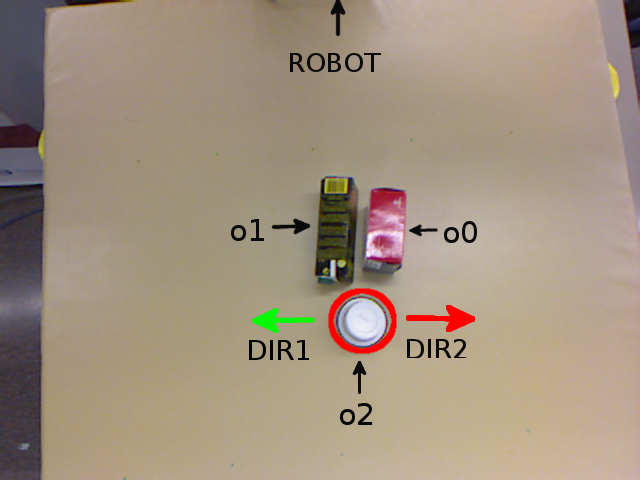
\includegraphics[width=5cm]{Img/backtracking/image4.png}
\caption{Unfeasible plan due to geometric constraints. In this case the planner returns as action to execute grasping or pushing away the white cup (highlighted by a red circle) but it is out the configuration space of the robot and there exist no plan for that problem. This problem is the one depicted in Figure \ref{fig:example_scene}, where the other objects has been grasped as consequence of the plan execution.} \label{fig:backtracking1}
\end{figure}

A situation in which the backtracking is useful is shown in Figure \ref{fig:backtracking1}. Accordingly to our strategy, the robot cannot be grasp the black or red box because the gripper would collide, and the same for the pushing action. It has to interact with the white cup in order to make space to move the other objects and then grasp them. The planner first returns the following plan: \texttt{(grasp o2)}, \texttt{(push\_dir1 o0)}, \texttt{(grasp o1)}, \texttt{(grasp o0)}. It will try to solve the inverse kinematic for the \texttt{(grasp o2)} action, but it found no solutions. Therefore the predicate \ttt{(ik\_unfeasible\_grasp o2)} is added and the planner replans. The new plan is: \texttt{(push\_dir1 o2)}, \texttt{(grasp o2)}, \texttt{(push\_dir1 o0)}, \texttt{(grasp o1)}, \texttt{(grasp o0)}. In this case it will try to get a solution for the inverse kinematic for the pushing action but it finds no solution, so the predicate \ttt{(ik\_unfeasible\_dir1 o2)} is added. And so on until the planner finds that all the possible actions for a feasible plan have no solutions for the inverse kinematic. In this way the planner includes the ability to understand also why there exist no plan for a certain problem. 

It may happen that the object outside the working space of the robot blocks the execution of the task because if the planner insists to return as first action an action with that object, then it will find that is not possible to interact with it and therefore there exist no solution on the planner procedure, this is the case previously presented. 
To overcome this, problem, and make the problematic objects left as the last one to interact with if possible, the actions are enhanced with another effect, that is all the objects that have one of the unfeasible inverse kinematic predicates set to true, are set to false. In this way, if possible, only the first action considers the geometric constraints, while the next ones have no information about the geometric constraints. 

\paragraph{PDDL}
For clarity purposes, the PDDL syntax of the described action is here reported. 
For the \textit{grasping} action its PDDL syntax is shown in listing \ref{graspPDDL}.

\lstset{language=pddl}
\begin{lstlisting}[caption={PDDL syntax of the grasping action},label=graspPDDL]
(:action grasp
    :parameters (?o - obj)
    :precondition (and
                  ; grasp it if there are no objects on its top
                  (not (exists (?x - obj)(on ?x ?o)))
                  ; grasp it if there is no object that blocks it
                  ; to be grasped
                  (not (exists (?x - obj)(block_grasp ?x ?o))))
    :effect (and
            ; the object "o" is grasped
            (grasped ?o)
            ; if the object was on top of other ones now it is
            ; no more on top of them
            (forall (?x - obj)
              (when (on ?o ?x) (not (on ?o ?x))))
            ; the grasped objects no more blocks other objects 
            ; to be pushed or grasped
            (forall (?x - obj)
              (when (block_grasp ?o ?x) (not (block_grasp ?o ?x))))
            (forall (?x - obj)
              (and
              (when (block_dir1 ?o ?x) (not (block_dir1 ?o ?x)))
              (when (block_dir2 ?o ?x) (not (block_dir2 ?o ?x)))
              (when (block_dir3 ?o ?x) (not (block_dir3 ?o ?x)))
              (when (block_dir4 ?o ?x) (not (block_dir4 ?o ?x))))
              ; remove all geometric constraints 
              (when (ik_unfeasible_dir1 ?x)(not (ik_unfeasible_dir1 ?x)))
              (when (ik_unfeasible_dir2 ?x)(not (ik_unfeasible_dir2 ?x)))
              (when (ik_unfeasible_dir3 ?x)(not (ik_unfeasible_dir3 ?x)))
              (when (ik_unfeasible_dir4 ?x)(not (ik_unfeasible_dir4 ?x)))
              (when (ik_unfeasible_grasp ?x)(not (ik_unfeasible_grasp ?x))))))
\end{lstlisting}

For the \textit{pushing} action its PDDL syntax is shown in listing \ref{pushPDDL}.

\lstset{language=pddl}
\begin{lstlisting}[caption={PDDL syntax of the pushing action along direction 1},label=pushPDDL]
(:action push_dir1
    :parameters (?o - obj)
    :precondition (and
                  ; push in direction 1 only if there are no
                  ; objects that block it along that direction
                  (not (exists (?x - obj)(block_dir1 ?x ?o)))
                  ; push it if it has no objects on top of it
                  ; and if it not on top of other ones
                  (not (exists (?x - obj)(on ?x ?o)))
                  (not (exists (?x - obj)(on ?o ?x))))
    :effect  (forall (?x - obj)
               (and
               ; once pushed the object is no more blocked in any direction
               ; and it no more blocks other objects to be moved
               (when (block_dir1 ?o ?x) (not (block_dir1 ?o ?x)))
               (when (block_dir2 ?o ?x) (not (block_dir2 ?o ?x)))
               (when (block_dir3 ?o ?x) (not (block_dir3 ?o ?x)))
               (when (block_dir4 ?o ?x) (not (block_dir4 ?o ?x)))
               (when (block_dir1 ?x ?o) (not (block_dir1 ?x ?o)))
               (when (block_dir2 ?x ?o) (not (block_dir2 ?x ?o)))
               (when (block_dir3 ?x ?o) (not (block_dir3 ?x ?o)))
               (when (block_dir4 ?x ?o) (not (block_dir4 ?x ?o)))
               ; once pushed it can be grasped and it no more
               ; blocks other objects to be grasped
               (when (block_grasp ?x ?o) (not (block_grasp ?x ?o)))
               (when (block_grasp ?o ?x) (not (block_grasp ?o ?x))))
               ; remove all geometric constraints 
               (when (ik_unfeasible_dir1 ?x)(not (ik_unfeasible_dir1 ?x)))
               (when (ik_unfeasible_dir2 ?x)(not (ik_unfeasible_dir2 ?x)))
               (when (ik_unfeasible_dir3 ?x)(not (ik_unfeasible_dir3 ?x)))
               (when (ik_unfeasible_dir4 ?x)(not (ik_unfeasible_dir4 ?x)))
               (when (ik_unfeasible_grasp ?x)(not (ik_unfeasible_grasp ?x)))))
\end{lstlisting}

\mbox{}


With such predicates the planner has all the basic information about the location of the objects on the scene. The symbolic predicates try to simplify the problem translating the geometric properties of the objects in symbolic ones. It is important to point out again that the system is deterministic, meaning that all the actions are supposed to give the resultant state with a probability of $1$. Clearly the more uncertainty is related to the pushing action, the direction selection, based on the principal axis, does not taken into account reliably the geometry of the object. The trajectory will be unlikely the desired one but a similar one. Overall the planner is considering to push the objects at infinity to isolate it, and that's false. This is another uncertainty of the pushing action due to the lack of geometric information. 
After the execution of an action the planner gets a new depth image from the Kinect, it segments the scene, it recomputes the predicates and replans. In this way the planner considers a totally new problem and all the uncertainties associated to the previous plan will be resolved to the current one. 
%In this manner we are forced to considered that some interactions between objects are allowed but tried to be avoid as much as possible. 

In order to provide a graphical scheme to the reader the planner pipeline is depicted in Figure \ref{fig:pipeline}. It can be appreciated the two fold strategy of the algorithm, the first stage (Figure \ref{fig:pipeline1}) is devoted to get the predicates from the Kinect sensor and the second one to evaluate the feasibility of the returned planned through backtracking and to execute the plan(Figure \ref{fig:pipeline2}).

\begin{figure}[t]
\centering
\begin{subfigure}[t]{\textwidth}
\centering
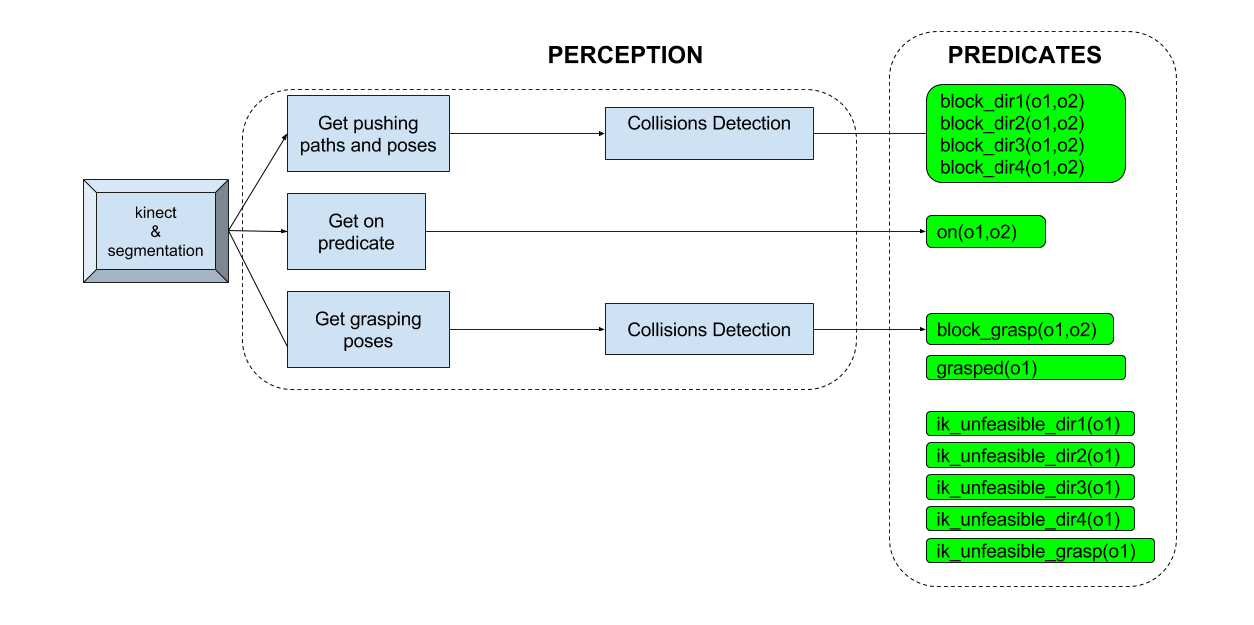
\includegraphics[width=\textwidth]{Img/planning/Pipeline1.png}
\caption{Perception Pipeline}\label{fig:pipeline1}
\end{subfigure}
\begin{subfigure}[t]{\textwidth}
\centering
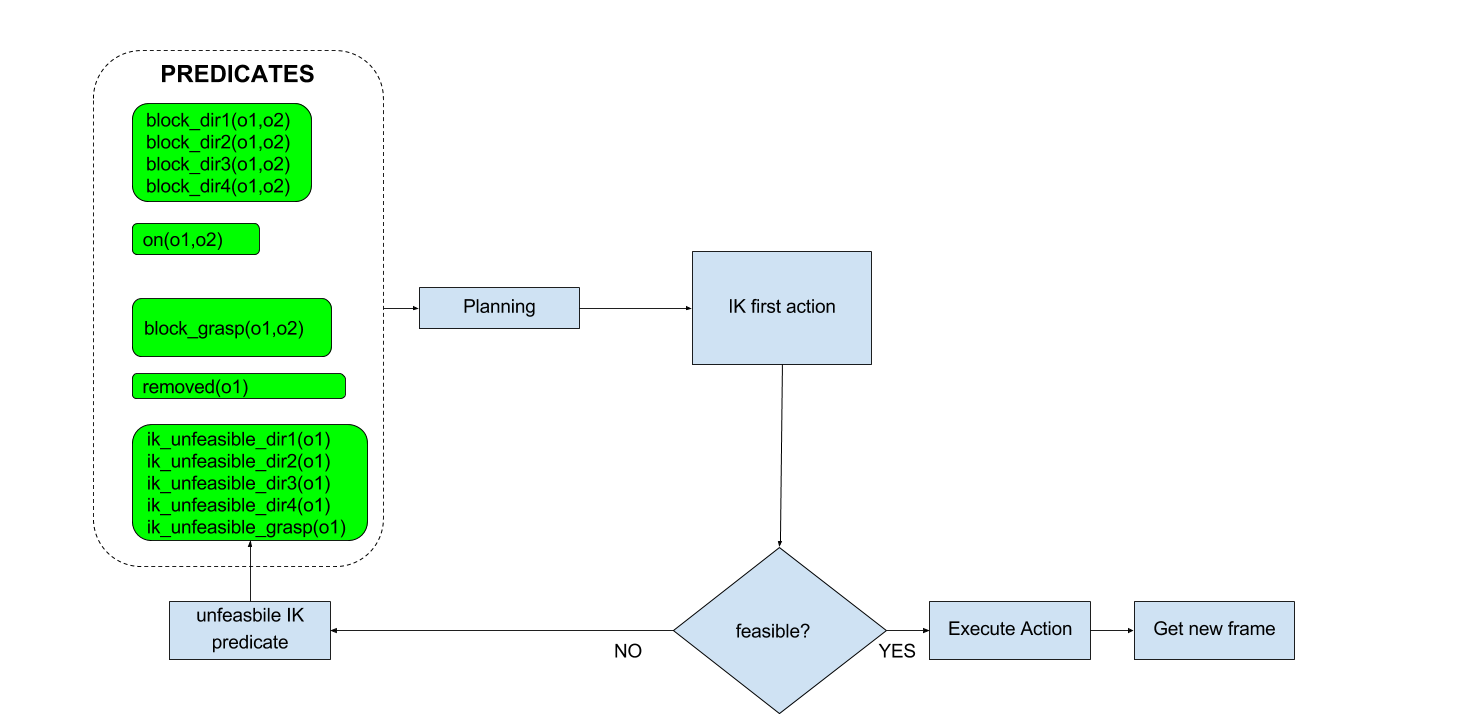
\includegraphics[width=0.9\textwidth]{Img/planning/Pipeline2.png}
\caption{Planning Pipeline}\label{fig:pipeline2}
\end{subfigure}
\caption{Planner pipeline}\label{fig:pipeline}
\end{figure}

Notice that the \ttt{grasped} predicate is just a predicate used only by the planner in order to know when the object has reached the goal or not, it does not need to be updated by the task planner. 

\mbox{}

How the predicates are computed will be discussed in detail in the next chapter.



